\documentclass[tikz,border=2pt]{standalone}
\usepackage{tikz}
\usetikzlibrary{arrows.meta,positioning}
\begin{document}
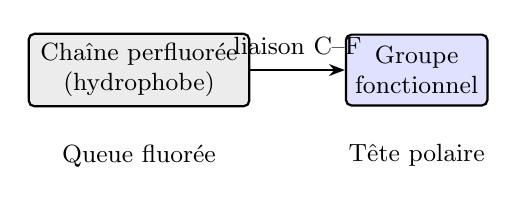
\begin{tikzpicture}[
    font=\small,
    >=Stealth,
    chain/.style={draw, thick, rounded corners=2pt, minimum height=0.9cm, minimum width=2.8cm, align=center},
    head/.style={draw, thick, fill=blue!12, rounded corners=2pt, minimum height=0.9cm, minimum width=1.6cm, align=center}
]
\node[chain, fill=gray!15] (chain) {Cha\^ine perfluor\'ee\\ (hydrophobe)};
\node[head, right=1.2cm of chain] (head) {Groupe\\ fonctionnel};
\draw[thick, -{Stealth[length=2mm]}] (chain.east) -- (head.west) node[midway, above=2pt] {liaison C--F};
\node[below=0.35cm of chain, align=center] {Queue fluor\'ee};
\node[below=0.35cm of head, align=center] {T\^ete polaire};
\end{tikzpicture}
\end{document}
